\documentclass{report}
\usepackage[utf8]{inputenc}
% \usepackage[hidelinks]{hyperref}
\usepackage{graphicx}
\usepackage{amsmath}
\usepackage{amssymb}
\usepackage{color}
\usepackage{pgfplots}

\graphicspath{ {./images/} }
\pgfplotsset{compat=1.16}
\usepgfplotslibrary{external}
\tikzexternalize[prefix=figures/]

\renewcommand\vec{\mathbf}
\newcommand{\norm}[1]{\left\lVert#1\right\rVert}
\newcommand*{\tran}{^{\mkern-1.5mu\mathsf{T}}}
\newcommand{\todo}{{\color{red} \textbf{TODO} }}

\newcommand{\quickwordcount}[1]{%
  \immediate\write18{texcount -1 -sum -merge #1.tex > #1-words}%
  \input{#1-words}words%
}
% \newcommand{\quickwordcount}[1]{X words}

\pgfdeclarelayer{pre main}
\begin{document}

\begin{titlepage}
    \centering
    
	{\scshape\LARGE Senior Honours Project\par}
	\vspace{0.25cm}
	{
\includegraphics[width=0.8\textwidth]{logo.png} \par}
    \vspace{0.25cm}
	{\huge\bfseries Freeing Neural Training Through Surfing\par}
	\vspace{0.5cm}
	
    \vfill
    {\large \textit{Georg Wölflein\\170011885} \par}
	{\large \textit{Supervisor: Dr. Mike Weir} \par}
    
    \vspace{0.5cm}

    {April 9, 2020\par}

    \vfill
    
    Word count: \quickwordcount{report}
\end{titlepage}

\chapter*{Abstract}
\todo

\chapter*{Declaration}
``I declare that the material submitted for assessment is my own work except where credit is explicitly given to others by citation or acknowledgement.
This work was performed during the current academic year except where otherwise stated.
The main text of this project report is \quickwordcount{report} long, including project specification and plan.
In submitting this project report to the University of St Andrews, I give permission for it to be made available for use in accordance with the regulations of the University Library. 
I also give permission for the title and abstract to be published and for copies of the report to be made and supplied at cost to any bona fide library or research worker, and to be made available on the World Wide Web.
I retain the copyright in this work.''

\vspace{0.5cm}

\textit{Georg Wölflein}

\tableofcontents

\chapter{Introduction}
\textit{Describe the problem you set out to solve and the
extent of your success in solving it. You should include
the aims and objectives of the project in order of
importance and try to outline key aspects of your
project for the reader to look for in the rest of your
report.}
\todo

\chapter{Context survey}
\textit{Surveying the context, the background literature and
any recent work with similar aims. The context survey
describes the work already done in this area, either as
described in textbooks, research papers, or in publicly
available software. You may also describe potentially
useful tools and technologies here but do not go into
project-specific decisions.}
\begin{itemize}
    \item TensorFlow
    \item keras
\end{itemize}
\todo

\chapter{Requirements specification}
Primary objectives:
\begin{enumerate}
    \item Design a generic framework that can be used for various neural training algorithms
    with a clear set of inputs and outputs at each step. This framework should include
    benchmarking capabilities.
    \item For a simple case of this framework (when the dimensionality of the control space
    and output space are suitably low), implement a visualisation tool that shows the
    algorithm’s steps.
    \item Implement a particular training algorithm for the framework that uses potential field
    techniques.
    \item Evaluate the performance of this and other algorithms on tasks of differing
    complexity, especially with regard to the local minimum problem and similar issues.
\end{enumerate}
Secondary objectives:
\begin{enumerate}
    \item Investigate how this approach can be generalized to any numerical optimisation problems.
\end{enumerate}

\section{Ethics}
There are no ethical considerations. 
All questions on the preliminary self-assessment form were answered with ``NO'' and hence no ethics form had to be completed.

\chapter{Theory}
\section{Supervised learning}

\paragraph{Regression model}
In machine learning, a regression model $f$ is defined as a mathematical function of the form
\begin{equation}
    \label{eq:reg_model}
    f(\vec{x}) = \hat{y} = y + \epsilon
\end{equation}
that models the relationship between a $D$-dimensional feature vector $\vec{x} \in \mathbb{R}^D$ of independent (\textit{input}) variables and the dependent (\textit{output}) variable $y \in \mathbb{R}$. 
Given a particular $\vec{x}$, the model will produce a \textit{prediction} for $y$ which we denote $\hat{y}$.
Here, the additive error term $\epsilon$ represents the discrepancy between $y$ and $\hat{y}$.

\paragraph{Supervised learning}
A supervised learning algorithm for a regression task infers the function $f$ given in (\ref{eq:reg_model}) from a set of \textit{labelled training data}. This dataset consists of $N$ tuples of the form $\langle \vec{x}_i, y_i\rangle$ for $i=1,\dots,N$.
For each feature vector $\vec{x}_i$, the corresponding $y_i$ represents the observed output, or \textit{label} \cite{burkov2019}.
We use the vector
\begin{equation}
    \vec{y} = \begin{bmatrix}
        y_1 & y_2 & \cdots & y_N
    \end{bmatrix}\tran
\end{equation}
to denote all the labelled outputs in the dataset, and
\begin{equation}
    \vec{X} = \begin{bmatrix}
        \vec{x}_1 & \vec{x}_2 & \cdots & \vec{x}_N
    \end{bmatrix}\tran
\end{equation}
is the $N \times D$ matrix representing the corresponding feature vectors.

Similarly,
\begin{equation}
    \label{eq:sup_learn_prediction}
    \vec{\hat{y}} = \begin{bmatrix}
        \hat{y}_1 & \hat{y}_2 & \cdots & \hat{y}_N
    \end{bmatrix}\tran
\end{equation}
denotes a particular prediction for each training sample.

\section{Artifical neural networks}
Artifical neural networks (ANNs) take inspiration from the human brain and can be regarded as a set of interconnected neurons. 
More formally, an ANN is a directed graph of $n$ neurons (referred to as \textit{nodes} or \textit{units}) with weighted edges (\textit{links}).
Each link connecting two units $i$ and $j$ is directed and associated with a real-valued weight $w_{i,j}$. 

A particular unit $i$'s \textit{excitation}, denoted ${ex}_i$, is calculated as the weighted sum
\begin{equation}
    {ex}_i = \sum_{j=1}^n{w_{j,i} a_j} + b_i
\end{equation}
where $a_j \in \mathbb{R}$ is another unit $j$'s \textit{activation} and $b_i \in \mathbb{R}$ is the $i$th unit's \textit{bias}.
Notice that if there exists no link between unit $i$ and a particular $j$ then simply $w_{i,j}=0$ and therefore $j$ will not contribute to $i$'s excitation. 

The unit $i$'s activation is its excitation applied to a non-linear \textit{activation function}, $g$. We have
\begin{equation}
    \label{eq:ann_activation}
    a_i = g\left({ex}_i\right) = g\left(\sum_{j=1}^n{w_{j,i} a_j} + b_i\right).
\end{equation}
Activation functions will be explored in more detail in Section \ref{sec:activation_functions}. 


\paragraph{ANNs as regression models}
We can employ an ANN to model a regression problem of the form given in (\ref{eq:reg_model}). 
To do so, we need at least $D+1$ neurons in the network. 
We consider the first $D$ units to be the \textit{input} neurons, and the last neuron, $n$, is the output unit.
Furthermore, we require $w_{j,k}=0$ for $j,k \in \mathbb{Z}^+$ where $j \leq n$ and $k \leq D$ to ensure that there are no links feeding into the input neurons.

To obtain the prediction $\hat{y}$ given the $D$-dimensional feature vector $\vec{x}$, we set the activation of the $i$th unit to the value the $i$th element in $\vec{x}$ for $i=1,\dots,D$.
Then, we propagate the activations using (\ref{eq:ann_activation}) until finally the prediction is the activation of the last neuron, $\hat{y}=a_n$.
This process is often called \textit{forward propagation} or \textit{forward pass} \cite{russell2010}.

\paragraph{Single-layer perceptron}
A single-layer perceptron (SLP) is a type of ANN that consists of two layers, an input and an output layer.
Every input node is connected to every output node, but there are no intra-layer links (i.e. there are no links between any two input nodes or any two output nodes). 
This is what we call a \textit{fully-connected feedforward} architecture.
SLP architectures will always form a \textit{directed acyclic graph} (DAG) because there are no intra-layer or backwards connections.
Figure \ref{fig:single_layer_perceptron} an example of a DAG representing a SLP.

\begin{figure}[h]
    \begin{center}
        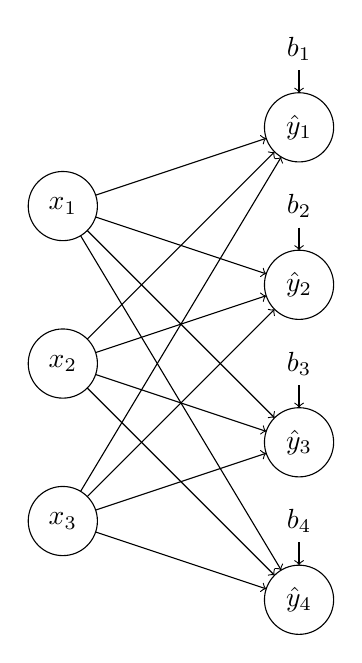
\begin{tikzpicture}
            [
                neuron/.style = {draw, circle, minimum size=25pt, inner sep=0pt, outer sep=0pt},
            ]
            \node [neuron] (x1) at (0,0) {$x_1$};
            \node [neuron] (x2) at (0,-2) {$x_2$};
            \node [neuron] (x3) at (0,-4) {$x_3$};
            \node [neuron] (n1) at (3,1)  {$\hat{y}_1$};
            \node [neuron] (n2) at (3,-1) {$\hat{y}_2$};
            \node [neuron] (n3) at (3,-3) {$\hat{y}_3$};
            \node [neuron] (n4) at (3,-5) {$\hat{y}_4$};
            \node (b1) at (3, 2) {$b_1$};
            \node (b2) at (3, 0) {$b_2$};
            \node (b3) at (3, -2) {$b_3$};
            \node (b4) at (3, -4) {$b_4$};
            \draw[->] (x1) -- (n1);
            \draw[->] (x1) -- (n2);
            \draw[->] (x1) -- (n3);
            \draw[->] (x1) -- (n4);
            \draw[->] (x2) -- (n1);
            \draw[->] (x2) -- (n2);
            \draw[->] (x2) -- (n3);
            \draw[->] (x2) -- (n4);
            \draw[->] (x3) -- (n1);
            \draw[->] (x3) -- (n2);
            \draw[->] (x3) -- (n3);
            \draw[->] (x3) -- (n4);
            \draw[->] (b1) -- (n1);
            \draw[->] (b2) -- (n2);
            \draw[->] (b3) -- (n3);
            \draw[->] (b4) -- (n4);
        \end{tikzpicture}
    \end{center}
    \caption{A single-layer perceptron with three input and four output neurons.}
    \label{fig:single_layer_perceptron}
\end{figure}

Let us consider a SLP with $m$ inputs and $n$ outputs. 
Since every output unit $i$ only has connections from every input unit $j$,
we can adapt (\ref{eq:ann_activation}) to give the activation of a particular output neuron $i$ as
\begin{equation}
    a_i = y_i = g\left({ex}_i\right) = g\left(\sum_{j=1}^m{w_{j,i} x_j} + b_i\right)
    = g\left( \vec{w}_i \vec{x}_i + b_i\right)
\end{equation}
where
$
    \vec{w}_i = \begin{bmatrix}
        w_{1,i} & w_{2,i} & \cdots & w_{m,i}
    \end{bmatrix}
$
represents the weights of all the edges that connect to output unit $i$.
If we use the $n \times m$ matrix
\begin{equation}
    \vec{W} = \begin{bmatrix}
        \vec{w}_1 \\ \vec{w}_2 \\ \vdots \\ \vec{w}_n
    \end{bmatrix} = \begin{bmatrix}
        w_{1,1} & w_{2,1} & \cdots & w_{m,1} \\
        w_{1,2} & w_{2,2} & \cdots & w_{m,2} \\
        \vdots & \vdots & \ddots & \vdots \\
        w_{1,n} & w_{2,n} & \cdots & w_{m,n}
    \end{bmatrix}
\end{equation}
to capture all weights and the vector $\vec{b} = \begin{bmatrix}
    b_1 & b_2 & \cdots & b_n
\end{bmatrix}\tran$ for the biases, we can give a mathematical formula describing the relationship between the inputs and outputs as
\begin{equation}
    \label{eq:single_layer_perceptron}
    \vec{f_{SLP}}(\vec{x}; \vec{W}, \vec{b}) = \vec{\hat{y}} = \vec{g}\left( \vec{W} \vec{x} + \vec{b} \right).
\end{equation}
Unlike the formula for a regression model, this is a vector-valued function, due to the fact that there are multiple outputs. 
Notice, however, that when $n=1$, we reach the same form as in (\ref{eq:reg_model}). 

\paragraph{Multi-layer perceptron}
A multi-layer perceptron (MLP) is a fully-connected feedforward ANN architecture with multiple layers which we will define in terms of multiple nested SLPs as in \cite{burkov2019}.
A MLP with $L$ layers is the mathematical function
\begin{equation}
    f_{MLP}(\vec{x})
        = \hat{y}
        = f_L \left(
            \vec{f}_{L-1} \left(
                \vec{\dots} \left(
                    \vec{f}_1 \left(
                        \vec{x}
                    \right)
                \right)
            \right)
        \right).
\end{equation}

Here, $\vec{f}_l(\vec{x}) = \vec{f_{SLP}}(\vec{x}; \vec{W}_l, \vec{b}_l)$ for $l = 1, \dots, L-1$. 
The outermost function $f_L$ is a scalar-valued function $f_L(\vec{x}) = f_{SLP}(\vec{x}; \vec{W}_L, \vec{b}_L)$ because it represents a SLP with one output unit which also means that $\norm{\vec{b}_L}=1$ and $\vec{W}_L$ has only one row.

The graph representing this network consists of connecting the outputs of the SLP representing layer $l$ with the inputs of the SLP representing layer $l+1$, as shown in Figure \ref{fig:multi_layer_perceptron}. 
The layers between the input and output layers are referred to as \textit{hidden} layers.

\begin{figure}[h]
    \begin{center}
        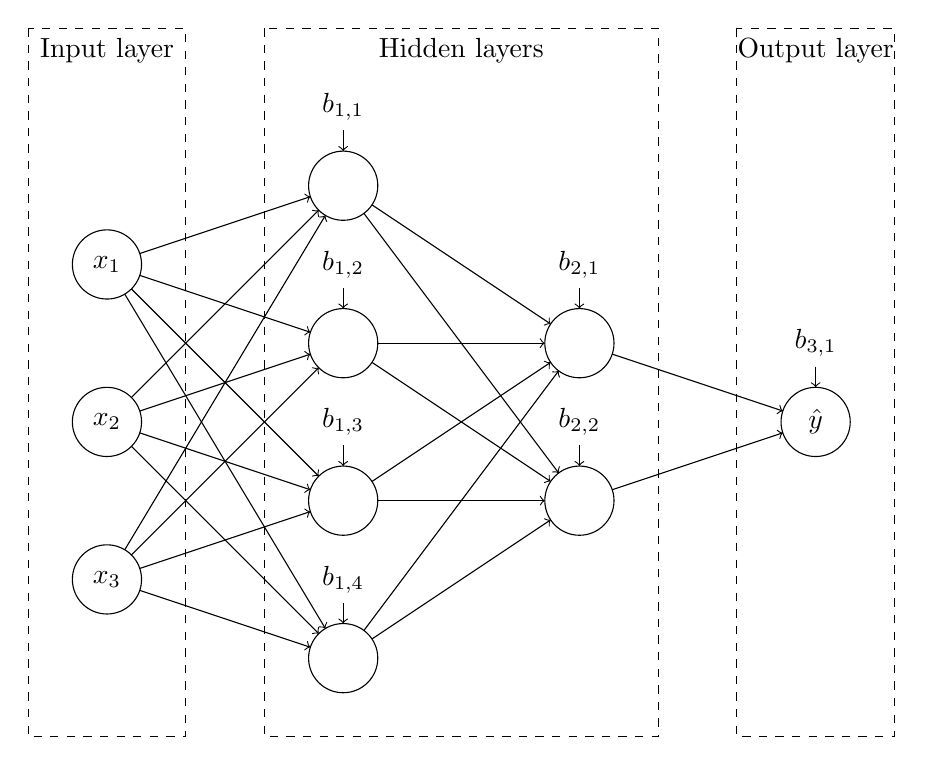
\begin{tikzpicture}
            [
                neuron/.style = {draw, circle, minimum size=25pt, inner sep=0pt, outer sep=0pt},
            ]
            \node [neuron] (x1) at (0,0) {$x_1$};
            \node [neuron] (x2) at (0,-2) {$x_2$};
            \node [neuron] (x3) at (0,-4) {$x_3$};
            \node [neuron] (h11) at (3,1) {};
            \node [neuron] (h12) at (3,-1) {};
            \node [neuron] (h13) at (3,-3) {};
            \node [neuron] (h14) at (3,-5) {};
            \node [neuron] (h21) at (6,-1) {};
            \node [neuron] (h22) at (6,-3) {};
            \node [neuron] (y) at (9, -2) {$\hat{y}$};
            \node (b11) at (3, 2) {$b_{1,1}$};
            \node (b12) at (3, 0) {$b_{1,2}$};
            \node (b13) at (3, -2) {$b_{1,3}$};
            \node (b14) at (3, -4) {$b_{1,4}$};
            \node (b21) at (6, 0) {$b_{2,1}$};
            \node (b22) at (6, -2) {$b_{2,2}$};
            \node (b3) at (9, -1) {$b_{3,1}$};
            \draw[->] (x1) -- (h11);
            \draw[->] (x1) -- (h12);
            \draw[->] (x1) -- (h13);
            \draw[->] (x1) -- (h14);
            \draw[->] (x2) -- (h11);
            \draw[->] (x2) -- (h12);
            \draw[->] (x2) -- (h13);
            \draw[->] (x2) -- (h14);
            \draw[->] (x3) -- (h11);
            \draw[->] (x3) -- (h12);
            \draw[->] (x3) -- (h13);
            \draw[->] (x3) -- (h14);
            \draw[->] (h11) -- (h21);
            \draw[->] (h11) -- (h22);
            \draw[->] (h12) -- (h21);
            \draw[->] (h12) -- (h22);
            \draw[->] (h13) -- (h21);
            \draw[->] (h13) -- (h22);
            \draw[->] (h14) -- (h21);
            \draw[->] (h14) -- (h22);
            \draw[->] (b11) -- (h11);
            \draw[->] (b12) -- (h12);
            \draw[->] (b13) -- (h13);
            \draw[->] (b14) -- (h14);
            \draw[->] (b21) -- (h21);
            \draw[->] (b22) -- (h22);
            \draw[->] (b3) -- (y);
            \draw[->] (h21) -- (y);
            \draw[->] (h22) -- (y);
            \draw[dashed] (-1,3) rectangle (1,-6);
            \draw[dashed] (2,3) rectangle (7,-6);
            \draw[dashed] (8,3) rectangle (10,-6);
            \node[below] (input) at (0,3) {Input layer};
            \node[below] (hidden) at (4.5,3) {Hidden layers};
            \node[below] (output) at (9,3) {Output layer};
        \end{tikzpicture}
    \end{center}
    \caption{A multi-layer perceptron with three inputs and two hidden layers.}
    \label{fig:multi_layer_perceptron}
\end{figure}

Since MLPs are simply nested SLPs, it follows that MLPs retain the DAG property and are therefore \textit{feedforward} networks as well.
In the forward pass, the activations are propagated from layer to layer (i.e. nested function to nested function) as in (\ref{eq:single_layer_perceptron}).

\section{Weight and output spaces}
We define the weight space $\mathcal{W}$ \todo

The output space $\mathcal{O}$ spans the space of all possible output predictions on the training set, $\vec{\hat{y}}$, so $\mathcal{O}=\mathbb{R}^N$ considering the fact that the training set has $N$ samples.

\section{Activation functions}
\label{sec:activation_functions}
Although units within a network can have different activation functions, this project solely employs networks where every unit uses the same $g$. 
Common activation functions include the sigmoid
\begin{equation}
    S(x) = \frac{1}{1 + e^{-x}}
\end{equation}
\todo

\chapter*{Ideas}
Generalize to classification as regression with multiple output variables?

\addcontentsline{toc}{chapter}{Bibliography}
\bibliographystyle{apalike}
\bibliography{bibliography}

\end{document}